\documentclass[11pt]{jsarticle}

% パッケージの宣言
\usepackage{url}
\usepackage{here}
\usepackage{natbib}
\usepackage{color}
\usepackage[dvipdfmx]{graphicx}
\usepackage{amsmath}
\usepackage{amsfonts}
\usepackage{amssymb}
\usepackage{bm}
\usepackage{multirow}
%\usepackage{tabudlarx}
\usepackage{latexsym}
\usepackage[dvipdfmx]{hyperref}
\usepackage{pxjahyper}

%argmax,argmin の定義
\DeclareMathOperator*{\argmin}{arg\,min}
\DeclareMathOperator*{\argmax}{arg\,max}



\title{購買行動及びブランド選択に対する広告の外部効果\\-ミクロデータによる消費者行動理論の解明-}
\author{網頭翔真 \thanks{慶應義塾大学経済学部3年} \and 藤本凌太朗 \thanks{同上} \and 坂本浩明 \thanks{同上} \and 打出紘基 \thanks{同上} \\ \and 須藤潤 \thanks{同上} \and 小林協介 \thanks{同上} \and 中村咲百合 \thanks{同上} \and 慶野有輝 \thanks{同上}\and 三田村豪太 \thanks{慶應義塾大学法学部政治学科}}

\begin{document}

\maketitle

 \thispagestyle{empty}

\begin{abstract}
本稿では、広告の外部効果による消費者の購買行動を解明することを目的とする。
従来の研究で定説とされきた他社の広告効果が自社商品の購買に負の影響を及ぼすことに疑問を呈し、カテゴリ購買とブランド選択という段階的になっている消費者の購買行動に競合他社の広告効果がどのような影響を及ぼしているのか、実データを用いた実証分析を行なった。\footnote{本稿の作成にあたっては、星野崇宏先生(慶應義塾大学経済学部)をはじめ、多くの方々から有益且つ熱心なコメントを頂戴した。ここに記して感謝の意を表したい。しかしながら、本稿にあり得る誤り、主張の一切の責任はいうま でもなく筆者たち個人に帰するものである。}\\[1ex] 
\end{abstract}

In this thesis, we propose the new analytical view of consumer behavior in terms of external advertisement influence by competitors. Many studies have been carried out in the field of advertising effectiveness. However, most of them only cover advertising effectiveness of one company on its own bland, and ignore the one of competitors. Even the limited thesis that includes the external advertisement influence by a competitor excessively simplifies an information processing by consumers and concludes that an advertisement by competitors has a negative influence on own companies’ bland purchase. However, taking a concept of category purchase and a positive contribution of advertisement to market itself  into consideration, it is rational to think about a possibility of positive advertisement effect of competitors on own bland. Therefore, based on the hypothesis that competitors’ advertisement can positively influence on own bland, we measured an advertising effectiveness with Poisson regression model as a first step. In a second step, we used a more advanced model to realize a simultaneous estimation of bland selection and category purchase. To sum up, we conclude that competitors’ television advertisement positively has an influence on own bland purchase.


\begin{center}
キーワード:外部効果、広告効果、ポアソン回帰、商品カテゴリー購買、複数ブランド選択、離散選択モデル、マルコフ連鎖モンテカルロ法、同時推定\\

\end{center}

\newpage

\pagenumbering{roman} % 目次はローマ数字
 \setcounter{tocdepth}{3}

\tableofcontents

\newpage
\pagenumbering{arabic}
 \setcounter{tocdepth}{3}


% ここから本文

\section{序論}
\label{ch:introduction}
本章では研究背景と研究目的、本稿の構成について述べる。
まず、\ref{sec:background}節で本研究を行うに至った背景を説明する。
次に、\ref{sec:previous_research}節で広告効果研究に関する先行研究を紹介し、その現状と問題点を指摘することで、本研究の背景と目的を述べる。
次に\ref{sec:constitution}節で本稿の構成を説明する。

\subsection{研究背景}
\label{sec:background}
本研究は、筆者の実体験に端を発した。 木枯らし吹き荒れる秋の家路を足早に進み帰宅した私は、身体に刷り込まれた動作のようにテレビリモコンを手に取り、何の気なしにテレビをつけた。テレビには温かいコーンポタージュのCMが流れており、冬の訪れを感じていた私にはとても惹かれるものがあった。翌日、より一層寒さが増す三田キャンパスで昨日のCMを思い出し、自動販売機の前へと歩みを進めた。マーケティングを学ぶ学生として「まんまとテレビ広告に訴求されてしまった。」と思いながらも、その手は止まることなくコーンポタージュのボタンに一直線に向かった。しかし、購入したコーンポタージュの缶で手を温めた後、ある一つの事実に気がつく。私が昨日見たテレビCMは、A社による広告であったが、手元にある缶はB社が販売するコーンポタージュだったのだ。通常広告とは、ある企業が自社の商品やブランドの認知・購買を促進するためのものであり、競合企業による広告は、自社の製品の売り上げなどに良い影響は及ぼさないと考えるのが妥当だろう。しかし、今回私はA社の広告により、B社の製品を購入していたのである。正確に言うならば、私は昨日に見たCMを、「A社のCM」ではなく、「コーンポタージュのCM」として認識していたのである。このような広告の認知の仕方は、広告の機能上ある意味合理的であり、私が行ったような一見非合理的な消費者の行動も奇異なものではないと言える。今回私が経験したこの実体験のように、競合企業による広告が自社製品の売り上げに貢献してしまっているという状況は多く存在するではないだろうか。こういった着眼点から、本論文では競合企業による広告の自社製品への正の影響、つまり正の広告外部効果について実証分析を行う。

\subsection{先行研究とその課題}
\label{sec:previous_research}
\citet{sunaga2008}は広告効果に関する研究を二つに大別した。
一つ目は消費者の行動的反応に焦点を当てた市場反応型の広告効果研究である。
これは主に、広告や価格を説明変数、売上、市場シェア、ブランド選択といった値を目的変数として、その直接的な関係について回帰分析やロジット・モデルを用いて説明を試みる研究である。
市場反応型の研究はさらに、扱うデータのタイプによって、集計レベルと個人レベルの2つの研究に分類することができる。集計レベルの研究とは、ブランドの広告支出、GRP、売上、市場シェアといったマーケット・データを用いた研究である。
一方、個人レベルの研究には、シングル・ソース・データを用いて個人や家庭に対する広告露出量とブランド選択の関係などの解明を試みる研究等がある。
具体的に市場反応型の広告研究を行った論文として、\citet{shimizu1990}のものが挙げられる。
これは、集計レベルの研究である。清水は、回帰式モデル、コイックラグ・モデル、山中モデル、広告ストック改良型モデルの4つのモデルをスーパーマーケットのチェーン店の週別、ブランド別売上高データに適用し、広告効果を測定した。
その結果、洗濯洗剤やカップヌードルなどの製品カテゴリにおいて、テレビ広告やラジオ広告が当該週の金額シェアに貢献していること、また、競合ブランドが存在する場合、ある特定ブランドの売上には、その競合ブランドの広告が影響を与えていることを示した。
個人レベルの市場反応型研究については、日本国内のデータを用いた研究は少なく、殆ど研究されていない。
集計レベル、個人レベルのいずれの市場反応型研究についても、その特徴として、消費者の行動的側面に焦点を当て、態度などの認知的な要素についてほとんど考慮していないことが挙げられる。
すなわち、消費者の処理プロセスをブラックボックス化、あるいは単純化して分析を行っている。

一方、広告効果研究の二つ目のタイプは、認知的反応型と呼ばれる。
広告効果の研究についてはこのタイプの研究が多くを占める。認知的反応型の研究とは、消費者の認知的反応に焦点を当て、消費者の内的な反応プロセスを捉えようとする研究である。
消費者の内的反応プロセスを説明するメカニズムとして、消費者のブランド認知次元を構造化したブランドカテゴライゼーションの概念が挙げられる。
以下は、\citet{brisoux1980}によるブランドカテゴライゼーションの概念図である。

\begin{figure}[htbp]
 \centering
 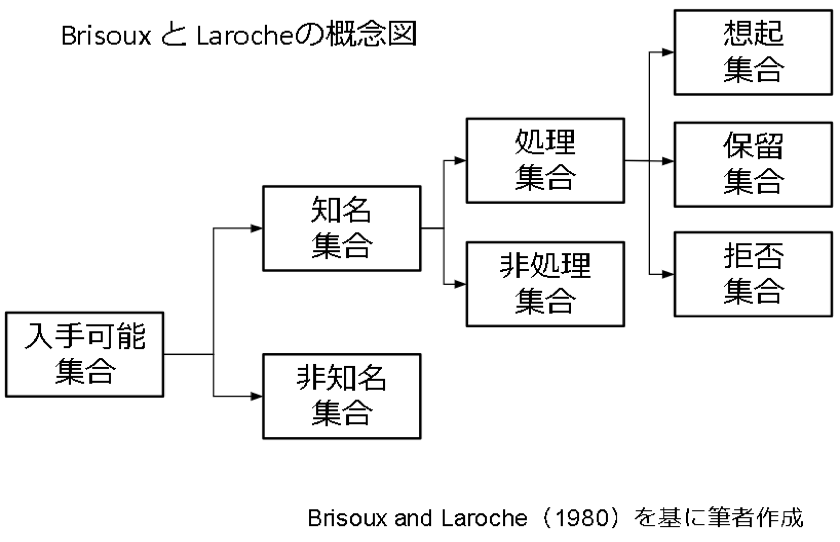
\includegraphics[width=10cm]{./fig/1-1_brand_categorization.png}
 \label{fig:brand_categorization}
\end{figure}

\newpage

\citet{brisoux1980}によれば、消費者は入手可能なブランドの中から名前を知っているブランドを知名集合として認識し、その中でも名前だけでなく、製品属性を知っているブランドを処理集合として認識する。
そして、処理集合の下位集合として、処理集合内のブランドを、好意的な態度を示している想起集合、中立的な態度を示す保留集合、否定的な態度を示す拒否集合の三つに分類する。
最後に、消費者は想起集合内の複数のブランドの中から購買するブランドを選択する。
したがって、購買候補となる想起集合の中に自社ブランドを組み込ませることが極めて重要となる。\citet{saito1999}は研究で、台所用洗剤に関するスキャナーパネルデータを用いて、上で述べた考慮集合を形成する際に、広告が正の効果を与えていることを示した。
さらに、\citet{saito1999}は、ロジットモデルと段階的ブランド選択モデルの結果を比較し、段階的ブランド選択モデルが考慮集合形成における広告効果研究に有用であると結論付けている。
ここで、\citet{urano2012}によれば、考慮集合と想起集合はほぼ同義である。
したがって、本稿でも考慮集合と想起集合について、同義として扱い議論している。\footnote{ブランドカテゴライゼーションに関する詳細な議論・定義に関しては、\citet{onzo1995}や\citet{katsumata2011}を参考にされたい。}

このように、広告についてはこれまで多くの議論がなされてきた。
市場反応型・認知的反応型のいずれの研究も、その多くが購買あるいはその認知的側面において、広告が正の効果を与えていると結論付けている。
しかし、一方で、認知的反応型の多くの分析は、競合企業の広告が自社ブランド選択にどのような影響を及ぼしているか検討していない。
一般的に、ある製品カテゴリには、複数のブランドが存在し、ブランド間で顧客を奪い合っている。
そのため、競合ブランドの広告が自社ブランドにどう影響しているか考慮する必要がある。

競合ブランドの広告が自社ブランドの購買行動に与える影響を考慮した数少ないものとして、上述の\citet{shimizu1990}の市場反応型研究の論文が挙げられるが、この論文に関しては別の問題点が存在する。
それは、集計レベルのマーケットデータを用いた分析のため、消費者の情報処理プロセスが単純化されており、広告がブランドに与える影響とカテゴリ全体に与える影響について分けて考慮されていない点である。
ある広告を見た際、消費者が皆等しく同一の次元でその広告を解釈するということは有り得ない。
そのため、解釈上の違いを考慮しなければ正確に広告効果を測定できているとは言えない。

また、産業組織論において、広告は消費者の需要、つまり当該カテゴリの消費量を増大させると説明している。\footnote{産業組織論における広告研究に関する詳細に関しては、\citet{uekusa2013}や\citet{nagaoka2013}を参考にされたい。}
このとき、広告によってもたらされたその需要の増加分は、単一ブランドの消費に帰するのではなく、ブランドシェアに広告によるインパクトを加えた形で複数のブランドに分配されることになるだろう。これはすなわち、競合企業の広告によっては、自社ブランドの売り上げが絶対値的に上昇する可能性があることを示す。産業組織論的観点から見た広告のこのような可能性は、上述したマーケティング上の広告研究には含まれておらず、考慮に入れる必要がある。

ここまで広告に関する先行研究の現状とその問題点について述べてきた。
一つ目は、広告効果研究において、競合企業の広告が及ぼす影響を考慮している研究が少ないという点。
二つ目は、競合企業の広告効果を考慮していたとしても、消費者によって広告の認識の仕方を一義的に捉えてしまっている点。
最後に、広告は消費者の需要を増大させるという産業組織論的視点が従来の広告研究に組み込まれていない点である。
以上の問題点に基づき、\ref{ch:hypothesis}章で本論文の仮説を提示する。


\subsection{本稿の構成}
\label{sec:constitution}
本稿の構成を以下に示す。
まず、\ref{ch:hypothesis}章では、\ref{sec:previous_research} 節で指摘した問題点を基に仮説を提示する。
\ref{ch:empirical_analysis}章では、実データを用いて仮説の実証を行う。
\ref{sec:empirical_summary}-\ref{sec:empirical_data}節では、今回使用する株式会社インテージ提供のパネルデータについて、その概要と変数の定義を述べる。
\ref{sec:poisson}節ではポアソン回帰を用いて、仮説を検証する。
\ref{sec:simultaneous_estimation_model}節では、カテゴリ購買とブランド選択の同時推定モデルを用いて、仮説をもう一段階精査し、議論を進める。
最後に、\ref{ch:conclusion}章で結論をまとめ、総括するとともに今後の展望を述べる。

\section{仮説の提示}
\label{ch:hypothesis}
本稿では、\ref{ch:introduction}章で述べた先行研究上の問題点から以下の仮説を提示する。それは、「競合他社の広告効果は、カテゴリ購買への正の効果と自社ブランド選択に対する負の効果をそれぞれ与える。その際、カテゴリ購買への正の影響が大きい場合は、自社の購買に正の外部効果を及ぼし、自社ブランド選択への負の影響が大きい場合には自社の購買に負の外部効果を及ぼす」というものである。

先述の\citet{shimizu1990}によると、競合ブランドの広告は、自社ブランドの購買に負の影響を与える。すなわち、競合ブランドの広告に接触すればするほど、自社のブランドは選択されなくなる。しかし、競合企業の広告がもたらす外部効果は、このような単純なものではない。実際には、競合企業の広告が、自社ブランドに与える外部効果と、カテゴリ全体に与える外部効果とに分けて考慮する必要がある。その理由は、研究背景で述べた例のように、消費者が競合企業の広告を見た際、それをブランドに対する広告ではなく、カテゴリに対する広告として認知することにより、製品カテゴリ自体の購買を促し、結果として自社ブランドの売り上げを絶対値的に上昇させる可能性があるからである。「企業の広告活動は、市場そのもの、製品カテゴリの需要を増大させる」という広告の産業組織論的解釈もこの議論を後押しするだろう。

そこで、本稿では、競合企業の広告の自社ブランドへの外部効果を
製品カテゴリ全体に対する需要、つまりカテゴリ購買に与える正の効果
自社ブランド選択に与える負の効果
の二つに区分する。
この前提に立てば、前者が後者を上回る場合は、自社の購買を促すという正の広告外部効果、後者が前者を上回る場合は、自社の購買を減ずるという従来考えられてきた負の広告外部効果の二つの外部効果が見出されるとの仮説が立てられる。

以下の章では、このような仮説について、株式会社インテージ提供のi-SSP(インテージシングルソースパネル)とSCI(全国消費者パネル調査)を用いた実証研究を行う。

この研究を行う意義として、従来のマーケティング広告効果研究に産業組織論の視点を加えた実証である点、競合ブランド広告の外部効果を二つに分けて理解することで、競合企業の広告を利用した最適な広告戦略の構築が可能になる点などが挙げられる。

従来の広告効果についての概念図と、本稿で提示した仮説の概念図は以下の通りである。

\begin{figure}[htbp]
 \centering
 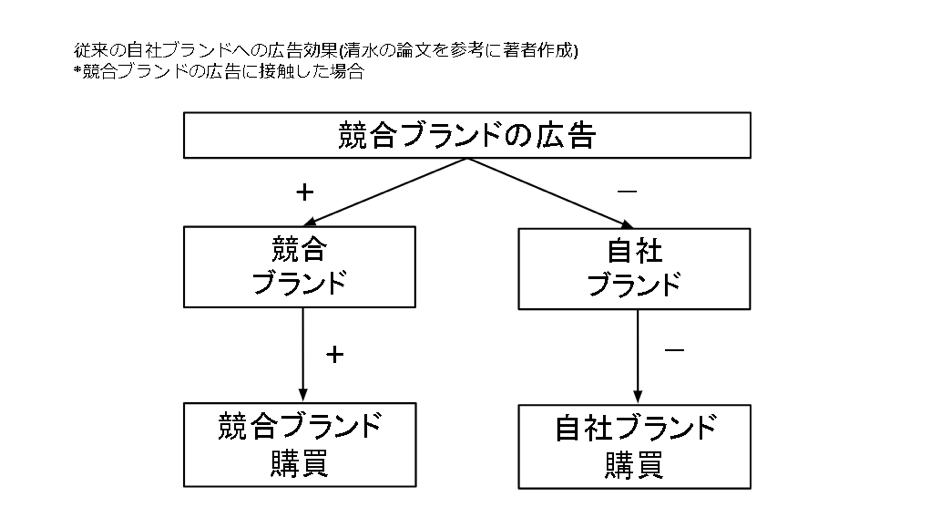
\includegraphics[width=11cm]{./fig/2_ad_before.png}
 \label{fig:ad_before}
\end{figure}

\begin{figure}[htbp]
 \centering
 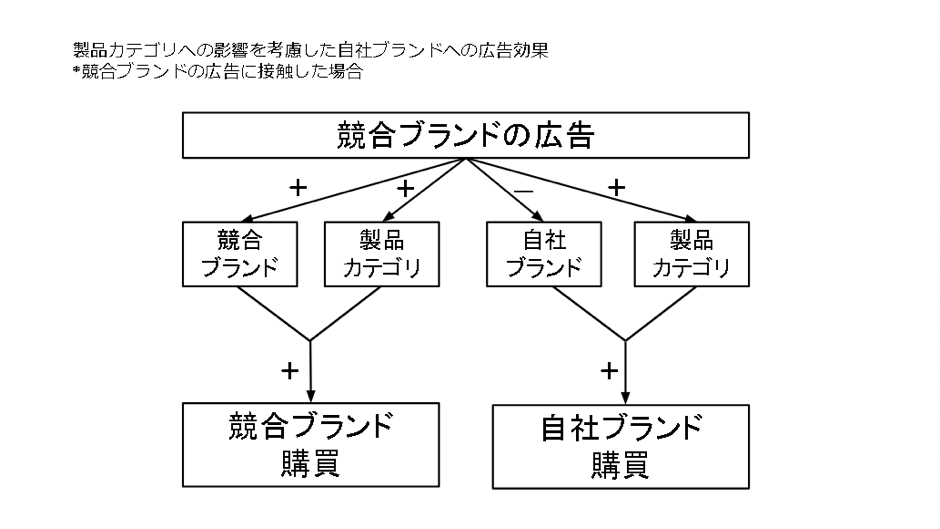
\includegraphics[width=11cm]{./fig/2_ad_after.png}
 \label{fig:ad_after}
\end{figure}


\section{実証分析}
\label{ch:empirical_analysis}

本章では、競合他社の広告効果が自社ブランドの商品購買に与える影響を検証する。
今回の検証では、広告のクロスメディア効果を証明することを趣旨としないため、データとして用いるのはテレビCMの接触データのみとする。
使用する広告データにテレビCMを選んだ理由は、他の広告媒体と比べ、各消費者ごとにパネルデータとして細かい頻度で集計することが可能であり、またWEBログなどと異なり、宣伝商品が明確であるため効果を測定しやすいことなどが挙げられる。
また、実証分析をする上での仮定として、一週間のテレビCMの合計接触回数が次の週における商品購買量に与える影響を証明することができれば、広告効果が商品購買に与える影響を証明できるとする。
\ref{sec:empirical_data}節では、本章で使用したデータの説明を行う。
\ref{sec:poisson}節では、ポアソン回帰モデルによる実証分析を行う。
\ref{sec:simultaneous_estimation_model}節では、同時推定モデルによる実証分析を行う。

\subsection{使用データ}
\label{sec:empirical_data}
本研究は、株式会社インテージ提供のi-SSP(消費者個人の広告接触に関するデータ)およびSCI(消費者個人の購買行動を記録したデータ)を使用している。提供データの詳細は付録を参照していただきたい。実証分析では、発泡酒の購買履歴にのみ注目する。その理由は大きく二つあり、一つ目は選択するブランドの数が限られていること、二つ目は外的要因により購買が影響されやすいことである。日本において発泡酒市場は寡占市場であり、消費者は無数のブランドから商品を選択するのではなく限られたブランドの中から効用の高い商品を選択する。また、発泡酒という財は各ブランドにおいて味や価格といった差異は小さく、ブランドイメージやディスプレイなどといった外的要因に購買行動が大きく影響されるという特徴がある。これら二つの理由から、広告効果の推定が行いやすいと考えられる発泡酒の購買データを利用した分析を行うこととする。本稿では、2014年1月1日から2015年12月31日の間で少なくとも一回以上発泡酒を購買している個人2,516サンプルのデータを抽出した。

今回の分析では、対象とする発泡酒のブランドを、ビールの市場シェア上位を占めるアサヒビール、キリンビール、サントリー、サッポロビールの4社が提供するブランド5つに絞ることとする。
それぞれ、クリアアサヒ(アサヒビール)、のどごし生(キリンビール)、淡麗(キリンビール)、金麦(サントリー)、麦とホップ(サッポロビール)の5つである。
キリンビールのみ2種類のブランドを分析対象としているが、これは消費者は発泡酒を購入する際に企業イメージを考慮せず、その商品に対するブランドイメージに基づいて購買をしているという仮説のもと分析を行なっているからである。
各ブランドにおける消費者の購買量、およびテレビCM接触回数の要約統計量は表\ref{tab:brand_summary1} に示す。
購買量の定義については、1単位を購入した個数とするため、350ml缶と500ml缶の購買はどちらも同じ1単位として集計している。
また、テレビCMの接触回数についても15秒や30秒といったCMの秒数は全て同じものとして扱い、テレビCMを見た場合に1回としてカウントする。

\begin{table}[htbp]
  \centering
  \caption{対象ブランドの概要}
\begin{center}
 \begin{tabular}{c|cccc|cccc} \hline
  \ & \multicolumn{4}{|c|}{\textgt{2年間の購買量}} & \multicolumn{4}{|c}{\textgt{1週間ごとの購買量}} \\
   & 平均 & 標準偏差 & 最小値 & 最大値 & \multicolumn{1}{|c}{平均} & 標準偏差 & 最小値 & 最大値 \\ \hline
   クリアアサヒ & 5 & 17.89 & 0 & 444 & 0.17 & 0.54 & 0 & 9 \\
   金麦 & 8.31 & 33.65 & 0 & 1082 & 0.27 & 0.75 & 0 & 17 \\
   淡麗 & 3.98 & 18.2 & 0 & 415 & 0.13 & 0.49 & 0 & 12 \\ 
   麦とホップ & 4.53 & 21.1 & 0 & 520 & 0.16 & 0.55 & 0 & 12 \\
   のどごし生 & 5.01 & 21.4 & 0 & 738 & 0.17 & 0.61 & 0 & 13 \\
   発泡酒全体 & 26.84 & 56.59 & 1 & 1082 & 0.9 & 1.22 & 0 & 21 \\
 \end{tabular}
 \label{tab:brand_summary1}
\end{center}
\end{table}

 \begin{center}
  \begin{tabular}{c|cccc|cccc} \hline
  \ & \multicolumn{4}{|c|}{\textgt{2年間のCM接触回数}} & \multicolumn{4}{|c}{\textgt{1週間ごとのCM接触回数}} \\
   & 平均 & 標準偏差 & 最小値 & 最大値 & \multicolumn{1}{|c}{平均} & 標準偏差 & 最小値 & 最大値 \\ \hline
  クリアアサヒ & 142.5 & 131.13 & 0 & 907 & 1.59 & 3.33 & 0 & 88 \\
  金麦 & 163.6 & 141.59 & 0 & 980 & 1.83 & 3.17 & 0 & 52 \\
  淡麗 & 99.31 & 91.86 & 0 & 614 & 1.13 & 2.4 & 0 & 38 \\
   麦とホップ & 63.16 & 57.14 & 0 & 387 & 0.71 & 1.68 & 0 & 28 \\
   のどごし生 & 117.2 & 106.39 & 0 & 721 & 1.31 & 2.43 & 0 & 45 \\
   発泡酒全体 & 669.5 & 590.37 & 0 & 4025 & 7.49 & 9.87 & 0 & 148 \\
 \end{tabular}
 \label{tab:brand_summary2}
\end{center}

(小数点以下第三位を四捨五入)

\subsubsection{ブランドロイヤリティの考慮}
\label{subsec:royality}
ブランドロイヤリティを考慮に入れることで、純粋な広告効果をより推定しやすくすることを目的とする。ブランドロイヤリティは個人の長期間における購買行動の結果と解釈し、提供データ2年間における分析対象5ブランドの購買割合と定義する。つまり、それぞれのブランドで購買割合が高いとロイヤリティが高い、購買割合が低いとロイヤリティが低いと言える。各個人の対象5ブランドにおける購買割合の合計値が1となるように数値化し、これをロイヤリティデータとして説明変数に用いる。例としてロイヤリティデータの構造を表\ref{tab:royality_ex} に示す。

\begin{table}[htbp]
  \centering
  \caption{ロイヤリティ}
\begin{center}
 \begin{tabular}{c|ccccc|c} \hline
   属性ID & クリアアサヒ & 金麦 & 淡麗 & 麦とホップ & のどごし生 & 計 \\ \hline
   1 & 0.125 & 0.313 & 0.062 & 0.375 & 0.125 & 1 \\
   2 & 0.08 & 0.42 & 0 & 0.06 & 0.42 & 1 \\
   3 & 0.12 & 0 & 0 & 0.88 & 0 & 1 \\
   ・ & ・ & ・ & ・ & ・ & ・ & \\
   ・ & ・ & ・ & ・ & ・ & ・ & \\  
  \end{tabular}
  \label{tab:royality_ex}
 \end{center}
\end{table}

\subsubsection{消費者の属性データ}
\label{subsec:consumer_distribution}
分析対象である消費者の属性データの分布は表\ref{tab:consumer_distribution}\footnote{n=3407}に示す。
提供データより今回の論文に利用した属性情報は、発泡酒の購買量と強い相関を示した年代、性別、世帯年収、未既婚、世帯人数の5つである。
それぞれの回帰係数は表\ref{tab:distribution_dummy}\footnote{年代ダミー(20代=1、30代〜40代=2、50代以上=3)
性別ダミー(女性=0、男性=1)
世帯年収ダミー(700万円未満=0、700万円以上900万円未満=1、900万円以上=2)
世帯人数ダミー(1人=1、2人=2、3人以上=3)
未既婚ダミー(既婚=0、未婚=1)
とした。}に示す。
年代に関しては、30代〜40代の購買量が最も高く、次いで50代以上、20代以下となる。性別は男性の方が女性よりも購買量が高い。世帯年収は700万円〜899万円が最も購買量が高く、次いで699万円以下、900万円以上となる。これは、一定以上年収を超えると発泡酒よりもビールやワインなどの高級志向となるためと考えられる。世帯人数に関しては、単身世帯の購買量が最も高く、次いで三人世帯以上、二人世帯となる。既婚者よりも未婚者の方が購買量が高い。

\begin{table}[htbp]
 \centering
  \caption{属性情報の分布}
\begin{center}
 \begin{tabular}{c|ccc} \hline
   年代 & 20代 & 30代〜40代 & 50代 \\
    & 400 & 1739 & 1268 \\ \hline
   性別 & 男性 & 女性 &  \\
    & 1541 & 1866 &  \\ \hline
   世帯年収 & 〜699万 & 700〜899万 & 900万〜 \\
    & 2041 & 632 & 734 \\ \hline
   未既婚 & 未婚 & 既婚 &  \\
    & 898 & 2509 &  \\ \hline
   世帯人数 & 1人 & 2人 & 3人〜 \\
    & 444 & 854 & 2109 \\
   \end{tabular}
   \label{tab:consumer_distribution}
  \end{center}
 \end{table}
 
 \begin{table}[htbp]
 \centering
  \caption{属性データと発泡酒購買量}
\begin{center}
 \begin{tabular}{cc|c} \hline
  \multicolumn{2}{c|}{\textgt{属性}}  & \multicolumn{1}{c}{\textgt{回帰係数}} \\ \hline
  年代 & 30代〜40代ダミー & 25.96 *** \\
   & 50代〜ダミー & 19.32 *** \\ \hline
  性別 & 男性ダミー & 13.83 *** \\ \hline
  世帯年収 & 700〜899万ダミー & 22.84 *** \\
   & 900万〜ダミー & -12.86 *** \\ \hline
  世帯人数 & 1人ダミー & 17.45 *** \\
   & 2人ダミー & -12.89 *** \\ \hline
未既婚 & 未婚ダミー & 7.52 *** \\ \hline
   \end{tabular}
   \label{tab:distribution_dummy}
  \end{center}
 \end{table}
 
 ***は0.1%、**は1%、*は5%、.は10\%水準で統計的に有意であることを示す 。

\begin{figure}
 \begin{minipage}{0.5\columnwidth}
  \centering
  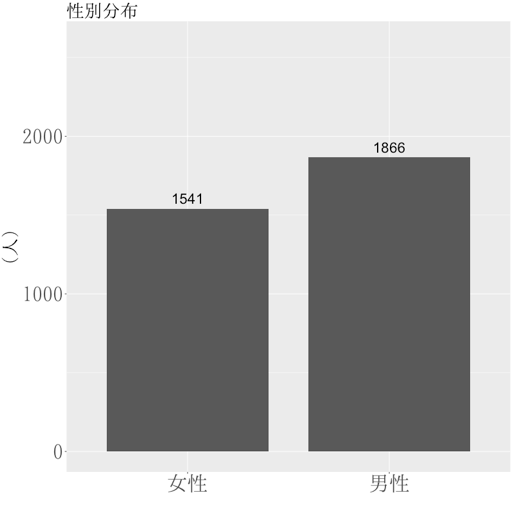
\includegraphics[width=\columnwidth]{./fig/3-2-2_seibetsu.png}
  \caption{性別}
  \label{fig:consumer_sex}
 \end{minipage}
 \begin{minipage}{0.5\columnwidth}
  \centering
  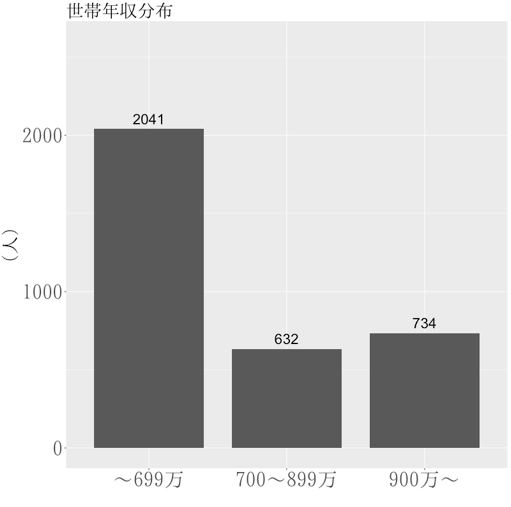
\includegraphics[width=\columnwidth]{./fig/3-2-2_nensyu.png}
  \caption{年収}
  \label{fig:consumer_annal_income}
 \end{minipage}
\end{figure}

\begin{figure}
  \centering
  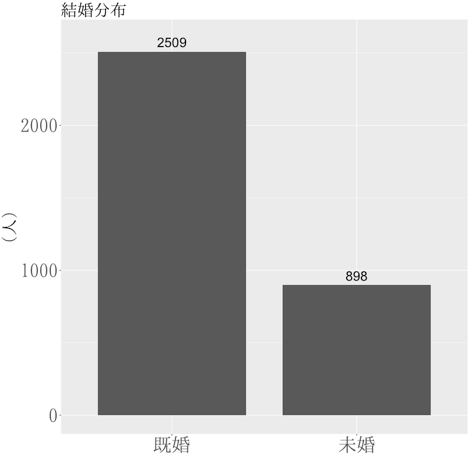
\includegraphics[width=8cm]{./fig/3-2-2_kekkon.png}
  \caption{結婚}
  \label{fig:consumer_marriage}
 \end{figure}
 
 \newpage
 
\subsection{ポアソン回帰モデル}
\label{sec:poisson}
この節では、自社ブランド商品の購買量を目的変数、自社及び競合他社のテレビCM接触回数を説明変数とした回帰分析により、競合他社の広告効果が自社ブランド商品の購買にどのような影響を与えているのかを検証する。
初めにポアソン回帰モデルの概要を紹介し、次に変数選択と推定、最後に結果と考察を行う。
この節の目的は、簡易的なモデルによる直感的な解釈をすることにあり、カテゴリ購買とブランド選択を同時推定した複雑なモデルに関しては\ref{sec:simultaneous_estimation_model}節で説明する。

\subsubsection{ポアソン回帰モデルの概要}
\label{subsec:poisson_summary}
ポアソン回帰とは、ポアソン分布をつかった統計モデルによるパラメータ推定を指す。
発泡酒iの購買量はカウントデータであるので、発泡酒iにおいて購買量がyである確率$p(y|\lambda)$はポアソン分布に従うとして、
\begin{equation}
 p(y|\lambda) = \frac{\lambda^{y}exp(-\lambda)}{y!}
\end{equation}
と仮定する。

ある発泡酒iの購買量の平均が
\begin{equation}
 \lambda_{i} = exp(\beta_{1} + \beta_{2}x_{i})
\end{equation}
このようにサイズ$x_{i}$を使ってかけると仮定し、両辺の対数をとると、
\begin{equation}
 \log (\lambda_{i}) = (\beta_{1} + \beta_{2}x_{i})
 \end{equation}
と書ける。

左辺はlink関数、右辺は線形予測子と呼ばれ、link関数はlog link関数で線形予測子は$z = \beta_{1} + \beta_{2}x_{i}$となっている。
ここでlog link関数を用いるのは、計算に都合よく、かつわかりやすいからである。
ポアソン分布の平均パラメータ$\lambda_{i}$は常に$\lambda_{i} > 0$でなければならない。
$\lambda_{i} = exp(z_{i})$というように線形予測子$z = \beta_{1} + \beta_{2}x_{i}$を$exp()$で囲っておくことで$z$がどのような値をとっても$\lambda_{i}$は常に非負の値となる。

確率分布の平均を$\lambda_{i} = exp(\beta_{1} + \beta_{2}x_{i})$と決めたので、ある発泡酒iで購買量が$y_{i}$である確率はポアソン分布の確率密度関数を使って、

\begin{equation}
 p(y_{i}|\{\beta_{j}\}, \{x_{i}\}) = \frac{\lambda^{y_{i}}_{i}exp(-\lambda_{i})}{y_{i}!}
\end{equation}
と書ける。全個体の尤度は
\begin{equation}
 L( \{ \beta_{i} \} | \{y_{i} \}, \{ x_{i} \} ) = \prod_{i = 1}^{N} \frac{\lambda^{y_{i}}_{i}exp(-\lambda_{i})}{y_{i}!}
\end{equation}
対数尤度は

\begin{equation}
 \log L( \{ \beta_{i} \} | \{y_{i} \}, \{ x_{i} \} ) = \sum_{i = 1}^{N} \log \{ \frac{\lambda^{y_{i}}_{i}exp(-\lambda_{i})}{y_{i}!} \}
\end{equation}
であり、これを最大化するような$\hat{\beta_{1}}$と$\hat{\beta_{2}}$を求めることをポアソン回帰という。


\subsubsection{変数選択と推定}
\label{subsec:poisson_variable}
実証分析を行うにあたりポアソン回帰モデルを選択した理由は、目的変数である発泡酒の購買量がカウントデータであり、ポアソン分布が最も当てはまりが良いためである。
目的変数の分布は表\ref{tab:law-molt_beer_frequency_distribution_rate}に示す。
実証分析に使用したデータに関しては\ref{sec:empirical_data}節で取り上げたが、モデルとの当てはまりを考慮し、季節効果を除去するために2015年7月から8月の間の4週間のデータのみを使用して分析を行う。
また、広告の接触回数は0から1に正規化したものを説明変数として用いた。
この期間での広告接触データと購買データが有効なサンプル数は1,511である。
モデルに利用した説明変数の一覧は表\ref{tab:explanatory_variable_description}に示す。自社ブランドのCM接触回数と他社ブランドのCM接触回数に関しては明らかな相関があるため、別のモデルとして組み込むこととする。
ビールカテゴリの合計CM接触回数を説明変数に入れている理由は、発泡酒とビールを完全に区別していない消費者がビールカテゴリのCMに触発されて購買行動を起こす可能性を考慮しているためである。
また、変数の選択に関しては、CM接触回数は固定とし、他の変数はステップワイズ法を用いて決定した。

\begin{table}[htbp]
 \centering
  \caption{発泡酒購買量の度数分布表}
\begin{center}
 \begin{tabular}{c|ccccccccccccc} \hline
  & 0 & 1 & 2 & 3 & 4 & 5 & 6 & 7 & 8 & 9 & 10 & 11 & 12 \\ \hline
  クリアアサヒ & 4001 & 562 & 96 & 28 & 8 & 4 & 2 & 4 & 0 & 2 & 0 & 0 & 0 \\
  金麦 & 3882 & 644 & 108 & 44 & 6 & 5 & 15 & 2 & 0 & 0 & 0 & 0 & 1 \\
  淡麗 & 4301 & 309 & 58 & 27 & 7 & 4 & 1 & 0 & 0 & 0 & 0 & 0 & 0 \\
  麦とホップ & 4247 & 346 & 60 & 22 & 5 & 6 & 11 & 6 & 3 & 1 & 0 & 0 & 0 \\
  のどごし生 & 4066 & 495 & 99 & 24 & 9 & 6 & 6 & 2 & 0 & 0 & 0 & 0 & 0 \\
 \end{tabular}
 \label{tab:law-molt_beer_frequency_distribution_rate}
 \end{center}
\end{table}

\begin{table}[htbp]
 \centering
  \caption{説明変数一覧}
\begin{center}
 \begin{tabular}{c|c} \hline
  \multicolumn{1}{c|}{\textgt{説明変数}} & \multicolumn{1}{c}{\textgt{内容}} \\ \hline
  自社ブランドのCM接触回数 & 一週間における特定ブランドのCM接触の回数 \\ 
   & (0から1に正規化したものを使用)\\
  他社ブランドのCM接触回数 & 一週間における特定ブランド以外の発泡酒の合計CM接触回数 \\
   & (0から1に正規化したものを使用)\\
  ビールカテゴリのCM接触回数 & 一週間におけるビールカテゴリの合計CM接触回数 \\
   & (0から1に正規化したものを使用)\\  
  特定ブランドのロイヤリティ & \ref{subsec:royality}項を参照。 \\
  年代 & 年代ダミー(20代=1、30代〜40代=2、50代以上=3) \\
  性別 & 性別ダミー(女性=0、男性=1) \\
  世帯年収 & 世帯年収ダミー \\
   & (700万円未満=0、700万円以上900万円未満=1、900万円以上=2) \\
  世帯人数 & 世帯人数ダミー(1人=1、2人=2、3人以上=3) \\
  未既婚 & 未既婚ダミー(既婚=0、未婚=1) \\
 \end{tabular}
 \label{tab:explanatory_variable_description}
 \end{center}
\end{table}

{\bf ステップワイズ法}\\
ステップワイズ法とは、回帰分析における変数選択法の一つである。
ステップワイズ法を行う手順は以下の通りである。
(1). 初期モデルを作成する。(2). AIC(赤池情報量規準)が最も小さくなるように変数を一つずつ追加もしくは削除をする。(3). AICを改善できなくなるまで(2)を繰り返す。
今回はこのような手法により変数の選択を行なった。

\subsubsection{結果と解釈}
ポアソン回帰分析による推定結果は表\ref{tab:poisson_result}に示す。
この結果から、発泡酒5ブランド中3ブランド(クリアアサヒ、淡麗、麦とホップ)に関しては自社ブランドのCM接触回数が購買に対して1\%〜10\%水準で有意に正の影響を与えていることがわかる。
また、この3ブランドに関しては競合他社のCM接触回数も自社ブランド商品購買に対して1\%〜5\%水準で有意に正の影響を与えていることがわかる。
他2ブランドに関して、まず金麦については、競合他社のCM接触回数が負の影響を与えているが、自社のCM接触回数も同じく負の影響を与えており、直感とは異なる結果が得られたため、考慮しきれていない説明変数によってうまく推定が行えていない可能性がある。次にのどごし生についても、有意な差を得られなかったため、今回のモデルでは説明が不十分であった。
しかし、5ブランド中3ブランドでは推定がうまく行えていることから、この結果を今回の推定の結論として用いることとする。
つまり、本稿では競合他社の広告効果は自社ブランドの商品購買に正の影響を与えると結論づける。
この結果が得られた要因を考察すると、消費者の購買行動はカテゴリ購買からブランド選択へと段階的になっているため、競合他社の広告接触がカテゴリ購買の段階で正に影響を与えることで自社のブランドの購買に対しても正の影響が検出されたと推測できる。
カテゴリ購買とブランド選択の同時推定モデルによる実証分析は\ref{sec:simultaneous_estimation_model}節で示す。

\begin{table}[htbp]
 \centering
  \caption{ポアソン回帰モデルの推定結果}
\begin{center}
 \begin{tabular}{c|ccc} \hline
  \multicolumn{1}{c|}{\textgt{目的変数}} & \multicolumn{3}{c}{\textgt{回帰係数}}  \\ \hline
   & 自社ブランドの & 他社ブランドの & ビールカテゴリの \\
   & CM接触回数 & CM接触回数 & CM接触回数 \\ \hline
  クリアアサヒの購買量 & 0.705 * & 1.20 *** & 1.79 *** \\
  金麦の購買量 & -0.406 & -0.838 * & -1.501 * \\
  淡麗の購買量 & 0.779 . & 0.966 * & 1.847 ** \\
  麦とホップの購買量 & 0.872 ** & 0.862 * & 1.584 *** \\
  のどごし生の購買量 & 0.026 & 0.34 & -0.009 \\
 \end{tabular}
 \label{tab:poisson_result}
 \end{center}
\end{table}

***は0.1%、**は1%、*は5%、.は10\%水準で統計的に有意であることを示す 。



\subsection{同時推定モデル}
\label{sec:simultaneous_estimation_model}
\ref{sec:poisson}節では、ポアソン回帰モデルを利用して自社及び他社の広告が購買にどのような影響を及ぼすかを推定した。この節ではこれをさらに発展し、自社と他社のテレビCM広告が、カテゴリ購買及びブランド購買に対してどのような影響を及ぼすのかを同時推定する。今回利用したモデルは、カテゴリー購買がブランド選択よりも先に起きるという仮定に基づいて、それらを同時推定するというものである。

\subsubsection{同時推定モデルの概要}
\label{subsec:simultaneous_summary}
a.カテゴリー購買\\
カテゴリーを選択したかを示す指示変数を$y_{it}$とする。ここで、$i$を個人、$t(t = 1,\ldots,T)$を購買機会とする。また、$v_{it}$をカテゴリー購買に対する潜在効用とし、これを説明変数$x$,変数の係数を$\beta$ とすると以下のようなモデルとして扱うことができる。ただし、潜在効用の回帰式での誤差項$\epsilon$は標準正規分布に従うと仮定する。\\
\begin{equation} \label{formulaa1}
y_{it} = \begin{cases}
             1 \;\; ( v_{it} > 0 )\\
             0 \;\; ( v_{it} \leq 0 )\\
             \end{cases}
             , \;\; v_{it} = \boldsymbol{x}^{\prime}_{it} \boldsymbol{\beta} + \epsilon_{it},
\end{equation}
\begin{equation} \label{formulaa2}
\epsilon_{it} \sim N(0, 1)
\end{equation}\\
\\
b.ブランド購買\\
$y_{itb}^{*}$をブランド$b(b = 1,\ldots,B)$を選択したかを示す指示変数とする。また、この指示変数を行列としたものを$\textbf{y}_{it}^{*} = (y_{it1}^{*},\ldots,y_{itB}^{*})’$とすると、これらの指示変数は以下のように示される。\\
\begin{equation} \label{formulab1}
y^\ast_{itb} = \begin{cases}
             1 \;\; ( u_{itb} \geq 0 \;\; \mbox{or} \;\; \mbox{argmax}_{k}u_{itb} = b)\\
             0 \;\; ( u_{itb} < 0 \;\; \mbox{and} \;\; \mbox{argmax}_{k}u_{itb} \neq b)\\
             \end{cases}
\end{equation}\\
さらに、ブランド$b$に対する潜在効用を$u_{itb}$とし、説明変数を$W_{it}$、変数の係数を$\gamma$ とする。このとき、ブランドの潜在効用の行列を$\textbf{u}_{it} = (u_{it1}^{*},...,u_{itB}^{*})’$とする。ただし、個人差を考慮するために$W_{it}$は単位行列と説明変数を含む列ベクトルを並べたような形状になる。説明変数には、自社の広告接触回数、他社の広告接触回数、年収や年齢等のデモグラフィック変数が含まれる。$OW = 自社の広告接触回数(own conpany)$、$OT = 他社の広告接触回数(other conpany)$、$B = ブランドロイヤリティ$として、これらを以下のように示す。\\
\begin{equation} \label{formulab2}
\textbf{u}_{it} = W_{it}\gamma + \delta_{it}
\end{equation}\\
\begin{equation} \label{formulab3}
  W_{it} =
  \begin{pmatrix}
      1 & 0 & 0 & \ldots & 0 & OW_{it1} & OT_{it1} & B_{it1} \\
      0 & 1 & 0 & \ldots & 0 & OW_{it2} & OT_{it2} & B_{it2} \\
       &  & \vdots &  &  & \vdots & \vdots & \vdots \\
      0 & 0 & 0 & \ldots & 1 & OW_{itB} & OT_{itB} & B_{itB}
    \end{pmatrix}
    ,
\end{equation}\\
\begin{equation} \label{formulab4}
  \boldsymbol{\gamma} =
  \begin{pmatrix}
      \gamma_{it1} & \ldots & \gamma_{B} & \gamma_{OW} & \gamma_{OT} & \gamma_{B}
   \end{pmatrix}
\end{equation}\\
\\
c.潜在効用の同時分布\\
カテゴリ購買の潜在効用$v_{it}$とブランドの潜在効用$\textbf{u}_{it}$の同時分布を以下のように仮定する。\\
\begin{equation} \label{formulac1}
  \begin{pmatrix}
      v_{it} \\
      \textbf{u}_{it} 
   \end{pmatrix}
   \sim N
  \begin{pmatrix}
    \begin{pmatrix}
    \boldsymbol{x}^{\prime}_{it}\boldsymbol{\beta}\\
    W_{it}\gamma
    \end{pmatrix}
    ,
    \begin{pmatrix}
    1 & {\boldsymbol \rho}^\prime\\
    {\boldsymbol \rho} & \Psi + {\boldsymbol \rho} \cdot {\boldsymbol \rho}^\prime
    \end{pmatrix}
  \end{pmatrix}
\end{equation}\\
この時、${\boldsymbol \rho}$は$v_{it}$と$\textbf{u}_{it}$の各要素の共分散ベクトル、$\Psi$ は$v_{it}$が所与である時の$\textbf{u}_{it}$の分散共分散行列である。
この同時分布の注意点としては、カテゴリーが非購買である時は必然的にそのカテゴリーに含まれるブランドは購買されないので、$\textbf{u}_{it}$は存在しない。これは、ブランド選択よりカテゴリー選択が先に起きるという仮定に基づいている。\\
また、消費者$i$の購買数を$\textbf{Q}_{it} = (Q_{it_{1}}, \ldots, Q_{itb})'$とすれば、 \\
\begin{equation}
Q_{itm} \leq Q_{itn} \iff u_{itm} \leq u_{itn}
\end{equation}\\
が成り立つ。これにより、推定した潜在効用から購買量の大小関係を把握することができる。
\\
d.尤度\\
<d-1>完全データの尤度\\
まず、指示変数$\textbf{y}_{it}^{*}$に欠損値がない場合をについての尤度を示す。
カテゴリー購買の潜在効用$v_{it}$に関するパラメーターを$\Theta_{v}$、ブランド購買の潜在効用$\textbf{u}_{it}$に関するパラメーターを$\Theta_{u}$とする。$v_{it}$が所与の時、 \\
\begin{equation} \label{formulad1}
R_{it} = 
\begin{Bmatrix}
\textbf{u}_{it} : 
\begin{bmatrix}
u_{itb} \geq 0 \;\; \mbox{or} \;\; \mbox{argmax}_{k}u_{itk} = b \
(y^\ast_{itb} = 1) \
u_{itb} < 0 \;\; \mbox{and} \;\; \mbox{argmax}_{k}u_{itk} \neq b \
(y^\ast_{itb} = 0)
\end{bmatrix}
\end{Bmatrix}
\end{equation}\\
とすればブランド購買の指示変数の行列$\textbf{y}_{it}^{*}$の分布は、\\
\begin{equation} \label{formulad2}
p(y^\ast_{it} | v_{it}, \Theta_{u}) = \int_{R_{it}} p(\textbf{u}_{it} | v_{it}, \Theta_{u}) du_{it1} \ldots du_{itB}
\end{equation}\\
となる。
この時、尤度は以下のように示せる。
\begin{equation} \label{formulad1_1}
\begin{split}
L(\boldsymbol{y}, \boldsymbol{y^\ast} | \Theta_{v}, \Theta_{u}) &= \prod_{i=1}^{N} \prod_{t=1}^{T_{i}}
\begin{Bmatrix}
\int_{v_{it} \geq 0} p(y^\ast_{it} | v_{it}, \Theta_{u}) p(v_{it} | \Theta_{v}dv_{it})
\end{Bmatrix}^{y_{it}} \times \
\begin{Bmatrix}
\int_{v_{it} \geq 0} p(y^\ast_{it} | v_{it}, \Theta_{u}) p(v_{it} | \Theta_{v}dv_{it})
\end{Bmatrix}^{1 - y_{it}} \\
&= \prod_{i=1}^{N} \prod_{t=1}^{T_{i}}
\begin{Bmatrix}
\int_{v_{it} \geq 0} 
\begin{bmatrix}
\int_{R_{it}} p(v_{it}, \textbf{u}_{it} | \Theta_{v}, \Theta_{u}) du_{it1} \ldots du_{itB}
\end{bmatrix} dv_{it}
\end{Bmatrix}^{y_{it}} \\
& \quad \times \
\begin{Bmatrix}
\int_{v_{it} < 0} 
\begin{bmatrix}
\int_{R_{it}} p(v_{it}, \textbf{u}_{it} | \Theta_{v}, \Theta_{u}) du_{it1} \ldots du_{itB}
\end{bmatrix} dv_{it}
\end{Bmatrix}^{1 - y_{it}}
\end{split}
\end{equation}\\
\\
<d-2>完全尤度\\
欠測値を含むデータの解析を行う場合には完全尤度を利用する。完全尤度とは、完全データの尤度から欠測値を周辺化した尤度である。ブランド購買の観測部分を$y_{obs}^{*}$とすると、完全尤度は以下のように示される。\\
\begin{equation} \label{formulad2_1}
\begin{split}
L(\boldsymbol{y}, \boldsymbol{y}^\ast_{obs} | \Theta_{v}, \Theta_{u}) &=
\prod_{i=1}^{N} \prod_{t=1}^{T_{i}}
\left\{
\int_{v_{it} \geq 0} p(y^\ast_{it} | v_{it}, \Theta_{u}) p(v_{it} | \Theta_{u}) dv_{it}
\right\}^{y_{it}} \\
&\quad \times \left\{
\int_{v_{it} < 0} 
\left[_{all}
\sum_{\substack{y^\ast_{it1}, \ldots, y^\ast_{itB}}} p(y^\ast_{it} | v_{it}, \Theta_{u})
\right] p(v_{it} | \Theta_{u}) dv_{it}
\right\}^{1 - y_{it}} \\
&= \prod_{i=1}^{N} \prod_{t=1}^{T_{i}}
\left\{
\int_{v_{it} \geq 0}
\left[
\int_{R_{it}} p(v_{it}, \textbf{u}_{it} | \Theta_{v}, \Theta_{u}) du_{it1} \ldots du_{itB}
\right] dv_{it}
\right\}^{y_{it}} \\
& \quad \times \
\left\{
\int_{v_{it} < 0} p(v_{it} | \Theta_{v}) dv_{it}
\right\}^{1 - y_{it}}
\end{split}
\end{equation}\\
また、ブランド購買変数$y_{it}^{*}$の欠測値がランダムである場合、ブランド購買とカテゴリー購買が独立であるといえるため、${\boldsymbol \rho} = 0$ として、以下のように表現できる。\\
\begin{equation} \label{formulad2_2}
\begin{split}
L(\boldsymbol{y}, \boldsymbol{y}^\ast_{obs} | \Theta_{v}, \Theta_{u}, p = 0) &= \prod_{i=1}^{N} \prod_{t=1}^{T_{i}}
\left\{
\int_{v_{it} \geq 0} p(v_{it}) dv_{it}
\left[
\int_{R_{it}} p(\textbf{u}_{it} ) du_{it1} \ldots du_{itB}
\right]
\right\}^{y_{it}} \\
& \quad \times \
\left\{
\int_{v_{it} < 0} p(v_{it})dv_{it})
\right\}^{1 - y_{it}}
\end{split}
\end{equation}\\
\\
以上が尤度に関する部分であるが、実際の解析において最尤推定しようとすれば多数の積分により計算が複雑になるため、推定が困難になる。そこで、実際の推定ではマルコフ連鎖モンテカルロ方を用いて推定を行った。

\subsubsection{変数選択と推定}
\label{subsec:simultaneous_variable}
使用データは前節と同期間の購買データを利用し、カテゴリー購買の潜在効用とブランド選択の潜在効用を被説明変数としてそれぞれ表\ref{tab:simultaneous_category_variables}, \ref{tab:simultaneous_brand_variables}に示す変数を説明変数に用いた。

\begin{table}[htbp]
 \centering
  \caption{カテゴリ購買の潜在効用に関する説明変数}
\begin{center}
 \begin{tabular}{c|c} \hline
  \multicolumn{1}{c|}{\textgt{変数名}} & \multicolumn{1}{c}{\textgt{内容}} \\ \hline
 各発泡酒ブランドのCM接触回数 & 一週間における各発泡酒ブランドのCM接触の回数 \\
   & (0から1に正規化したものを使用) \\
 ビールカテゴリのCM接触回数 & 一週間におけるビールカテゴリの合計CM接触回数 \\
  &(0から1に正規化したものを使用) \\
 未既婚 & 未既婚ダミー(既婚=0、未婚=1) \\
 年代 & 年代ダミーとして30-40代ダミーと50代-ダミーを用意し、 \\
  & それぞれ(0, 1)で評価した。 \\
 性別 & 性別ダミー(女性=0、男性=1) \\
 世帯年収 & 世帯年収ダミーとして年収700-899万ダミーと \\
  & 年収900万-ダミーを用意し、それぞれ(0, 1)で評価した。 \\
 \end{tabular}
 \label{tab:simultaneous_category_variables}
 \end{center}
\end{table}

\begin{table}[htbp]
 \centering
  \caption{ブランド選択の潜在効用に関する説明変数}
\begin{center}
 \begin{tabular}{c|c} \hline
  \multicolumn{1}{c|}{\textgt{変数名}} & \multicolumn{1}{c}{\textgt{内容}} \\ \hline
  自社ブランドのCM接触回数 & 一週間における特定ブランドのCM接触の回数 \\
   & (0から1に正規化したものを使用) \\
  他社ブランドのCM接触回数 & 一週間における特定ブランド以外の発泡酒の合計CM接触回数 \\
   & (0から1に正規化したものを使用) \\
  特定ブランドのロイヤリティ & 各モニターについて、それぞれに観察された総購買機会の \\
   & 7割を超える割合で特定のブランドの単一購買が発生していた場合 \\
    & ”ロイヤリティあり”と判断し、(0, 1)で評価した。 \\
 \end{tabular}
 \label{tab:simultaneous_brand_variables}
 \end{center}
\end{table}

推定にはGibbs Sampler法を採用して5000回のサンプリングを行い、そのうち2000回をburn-inとして破棄した。
推定量としては平均値を採用した。

\subsubsection{結果と考察}
\label{subsec:simultaneous_result}
同時推定モデルによるパラメータ推定結果を以下に示す。
表\ref{tab:simultaneous_category_coef}のうちモニターのデモグラフィック情報に関する推定値を見ると、未婚や男性がカテゴリー購買に対して正に働き、高所得者(ビールを購買すると考えられる)は負に働いていることからこの推定値は直感に沿ったものであると言える。
その上で各CM接触の項目に着目すると、どのブランドのCMもカテゴリー購買に対して正の影響を与えていることがわかる。
また、ビールのCMもカテゴリー購買に対して正の影響を与えていることがわかる。
一方、表\ref{tab:simultaneous_brand_coef}の他ブランドCM接触の項目に着目すると、ブランド選択について他ブランドのCM接触は負の影響を与えていることがわかる。
以上の結果から、他ブランドや補完財(本実データ分析ではビール)のCM接触はカテゴリー購買に対して正の影響を与えるが、カテゴリー購買が発生した後のブランド選択の段階においては他ブランドのCM接触は自社ブランドの選択に対して負の影響を与えていると結論づけられる。
この結論は\ref{sec:poisson}節の結論を購買プロセスによって細分化して解析した結論といえ、同節の解析結果及び結論と連続性を持った結論であると言える。

また、この結論は、\citet{shimizu1990}が主張している「他社ブランドの広告は、自社ブランドの購買に負に影響を与える」という結論を実データを用いて否定することとなり、広告効果についての新たな知見を提供した。


\begin{table}[htbp]
 \centering
  \caption{カテゴリー購買に関する説明変数の係数}
\begin{center}
 \begin{tabular}{c|cc} \hline
\multicolumn{1}{c|}{\textgt{説明変数及び切片}} & \multicolumn{1}{c}{\textgt{係数推定値 }} & \multicolumn{1}{c}{\textgt{標準誤差}} \\ \hline
切片 & 0.049363888 & 0.000259853 \\
クリアアサヒCM & 0.002031096 & 0.000554629 \\
のどごし生CM & 0.003233694 & 0.000559359 \\
淡麗CM & 0.000852584 & 0.000550192 \\
金麦CM & 0.001745672 & 0.00056607 \\
麦とホップCM & 0.002156966 & 0.000569975 \\
ビールCM & 0.009624513 & 0.000494533 \\
未婚ダミー & 0.002866959 & 0.0001245 \\
世帯年収700~899万ダミー & 0.009593192 & 0.000121579 \\
世帯年収900万~ダミー & -0.004899229 & 0.000126453 \\
30~40代ダミー & 0.01866995 & 0.000188603 \\
50代ダミー & 0.013575297 & 0.000190871 \\
男性ダミー & 0.008435621 & 0.000106303 \\
 \end{tabular}
 \label{tab:simultaneous_category_coef}
 \end{center}
\end{table}

\newpage

\begin{table}[htbp]
 \centering
  \caption{ブランド選択に関する説明変数の係数}
\begin{center}
 \begin{tabular}{c|cc} \hline
  \multicolumn{1}{c|}{\textgt{説明変数及び切片}} & \multicolumn{1}{c}{\textgt{係数推定値}} & \multicolumn{1}{c}{\textgt{標準誤差}} \\ \hline
  クリアアサヒ切片 & 0.013643945 & 0.000291838 \\
  のどごし生切片 & 0.01094687 & 0.000286527 \\
  淡麗切片 & 0.007507617 & 0.000307929 \\
  金麦切片 & 0.013889913 & 0.000225938 \\
  麦とホップ切片 & 0.008677086 & 0.000221341 \\
  自ブランドCM接触 & 0.004861576 & 0.001975917 \\
  他ブランドCM接触 & -0.008771425 & 0.000837005 \\
  ブランドロイヤリティ & 0.078345802 & 0.000197288 \\
 \end{tabular}
 \label{tab:simultaneous_brand_coef}
 \end{center}
\end{table}

\begin{table}[htbp]
 \centering
  \caption{カテゴリー購買とブランド選択の潜在効用の誤差項に関する分散共分散行列}
\begin{center}
 \begin{tabular}{c|cccccc} \hline
   & カテゴリー & クリアアサヒ & のどごし生 & 淡麗 & 金麦 & 麦とホップ \\ \hline
カテゴリー購買 & 1 &  &  &  &  &  \\
   & (-) &  &  &  &  &  \\
クリアアサヒ購買 & 0.6180823 & 1 &  &  &  &  \\
 & (0.0106179) & (-) &  &  &  &  \\
のどごし生購買 & 0.5821811 & 0.415060 & 1 &  &  &  \\
 & (0.0111319) & (0.0111124) & (-) &  &  &  \\
淡麗購買 & 0.322499 & 0.2277351 & 0.2542587 & 1 &  &  \\
 & (0.0132428) & (0.0118378) & (0.0116131) & (-) &  &  \\
金麦購買 & 0.9752140 & 0.6151275 & 0.5800108 & 0.3224345 & 1 &  \\
 & (0.0007444) & (0.0103575) & (0.0108538) & (0.0129305) & (-) &  \\
麦とホップ購買 & 0.9766553 & 0.6160823 & 0.5802416 & 0.3231048 & 0.9604767 & 1 \\
 & (0.0007351) & (0.0103667) & (0.0108681) & (0.012951) & (0.0009544) & (-) \\
 \end{tabular}
 \label{tab:simultaneous_matrix}
 \end{center}
\end{table}
ただし、括弧内は標準誤差。

\begin{figure}[htbp]
 \centering
\begin{minipage}{0.6\columnwidth}
 \centering
 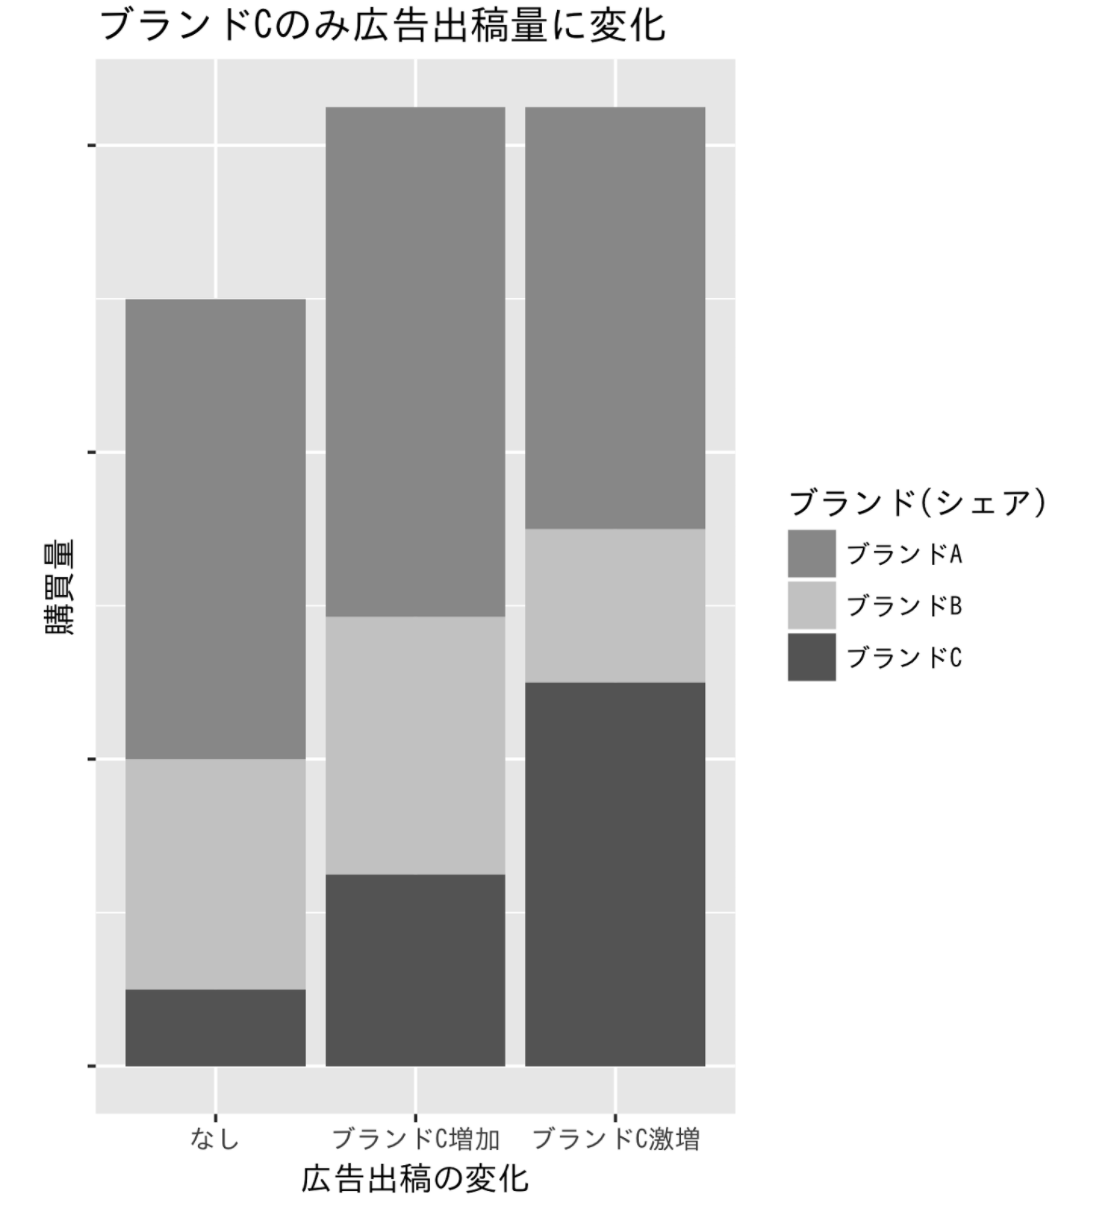
\includegraphics[width=\columnwidth]{./fig/3-4-3.png}
 \caption{広告出稿と購買量のシミュレーション}
 \label{fig:3-4-3}
\end{minipage}
\end{figure}

さらに、\ref{sec:poisson}節で得られた結果も踏まえ、これらの実データ解析の結論をマーケティング・広告戦略の観点から考察する。
ある商品カテゴリー業界はA, B, Cの3ブランドの寡占状態であるとすると、3社がどれも広告出稿量を変化させない状態での売り上げは図\ref{fig:3-4-3}左のグラフのようになっているとする。

ここで、ブランドCのみが広告出稿量を増加させた場合について考える。
まず、ブランドCの広告によるカテゴリー購買への正の効果がブランドA, ブランドBのブランド選択に与える負の効果を上回っている場合、それぞれの売上・シェアは図\ref{fig3-4-3}中央のグラフのように変動する。従来の理論ではブランドC以外の2ブランドはその売上を落とすと考えられてきたが、本実データ解析の結果からブランドCの広告の効果はカテゴリー購買の効用に正の影響を与えるという結論が得られており、商品カテゴリー全体の売上は増加し、これに伴って広告を発していないブランドA, ブランドBもその売上を若干伸ばすと考えられる。しかし、ブランド選択の段階においてブランドCの広告は自ブランドの選択のみに対して正の影響を与え、他2ブランドのブランド選択に対しては負の影響を与えるため、シェアの面ではブランドCのみがその割合を増やし、他2ブランドはシェアを落とすという結果になると考えられる。
次に、ブランドCの広告が大量に出稿されるなどして、ブランドCの広告によるカテゴリー購買への正の効果がブランドA, ブランドBのブランド選択に与える負の効果を下回っている場合、それぞれの売り上げ・シェアは図\ref{fig3-4-3}右のグラフのように変動する。前の例と同様にブランドCの広告はカテゴリー購買への需要を刺激し、カテゴリー全体の購買量は増加すると考えられる。しかし、このカテゴリー購買への正の影響よりも他2ブランドへのブランド選択段階での負の影響が大きいためブランドCの購買量が他2ブランドの購買量を奪い取る形で大きく伸びている。
このように本実データ解析の結果を踏まえると、広告戦略において他ブランド広告の売上面・シェア面の両面への効果と自ブランドの売上・カテゴリー内でのシェアを考慮した上での広告戦略を考えていくことができる。

\section{結論}
\label{ch:conclusion}
本章では、本稿で主張してきた論点を整理する。
まず、\ref{sec:conclusion}節では、前章の実証分析の結果を元に本稿の結論を述べる。
\ref{sec:issue}節では、実証分析で浮上した課題点についてまとめる。
最後に\ref{sec:suggestion}節では、本稿の主張の応用事例と今後の展望について述べる。

\subsection{結論}
\label{sec:conclusion}
本稿の結論は以下の通りである。

1.競合他社の広告が自社ブランドの購買に対し、カテゴリ購買の段階では正の影響を与え、ブランド選択の段階では負の影響を与えることを消費者個人のデータを用いた解析により実証した。

2.産業組織論的観点から見た広告効果が考慮された結論が実データにより導き出されており、競合他社の広告が自社ブランドの購買に正の外部効果を与える可能性があるという、従来仮説を反証する新たな知見を提示した。

\subsection{実証分析の課題}
\label{sec:issue}
本稿の実証分析では制約されたデータの中で実証を行なったためいくつかの課題が生じている。その中でも特に重要だと考える3つについてこの節で取り上げることとする。一つ目に新たな説明変数の必要性、二つ目にテレビCM以外の広告効果の検証、三つ目に別の製品カテゴリーによる検証について述べる。

\subsubsection{新たな説明変数の必要性}
\label{subsec:issue1}
本稿の実証分析、3.3節(ポアソン回帰モデル)では、発泡酒5ブランド中2ブランドでは有意な推定結果を得られることができなかった。その原因の一つに説明変数の不足が考えられる。今回取り入れた説明変数は、テレビCMの接触回数、ブランドロイヤリティ、属性情報のみであったが、実際の購買行動では、店舗での販売促進の有無、他ブランドとの価格差、ディスプレイの位置、パッケージデザインなどの変数が影響すると考えられる。これらの変数をモデルに適用することで、より精度の高い分析が行えると思われる。

\subsubsection{テレビCM以外の広告効果の検証}
 \label{subsec:issue2}
また、本稿の分析ではテレビCMのみを広告効果として考慮していたが、ダイレクトマーケティングやセグメントマーケティングなどを除いたマスマーケティングとしての広告であれば、本稿の結論と同じ結果が得られることが推測できる。
しかし、今回の実証分析ではテレビCM以外(新聞や雑誌、ラジオ、インターネットなど)の広告効果を検証することができなかったことが課題として残った。

\subsubsection{別の製品カテゴリーによる検証}
 \label{issue3}
本稿では、各ブランドに固有の差異が少なく、広告効果が推定しやすいと考えられる発泡酒という財のみで分析を行なったが、他社の広告効果が自社の商品購買に正の影響を与えるという結論が汎用的であるかどうかの検証を行うことができなかった。
発泡酒以外の製品カテゴリーでの実証分析を行うことで、本稿で得られた結論をより汎用的なものとしたい。

\subsection{今後の展望}
\label{sec:suggestion}
最後に今後の展望について述べ、本稿を締めくくる。この節では、消費者のブランド認知次元、実際の広告戦略の観点の二つについて述べる。まず、ブランド認知次元について、\citet{urano2012}で述べられているように、ブランドカテゴライゼーションでは考慮集合の定義や消費者による考慮集合の処理可能なサイズ、考慮集合形成のメカニズムや確率分布の応用など多くの研究が取り上げられている。しかし一方で、同等の位である拒否集合や保留集合に属するブランドに関しては注目がなされていない。もし消費者のブランドカテゴライゼーションを正確に把握することができれば、今回の実証分析の過程において、広告を出稿するブランドが消費者にとって拒否集合・保留集合・想起集合のどれに位置しているのかを考慮することができる。また、二つ目の広告戦略の観点より、競合他社の広告は自社の売上増加に寄与する反面シェアは低下するという、二つの効果を考慮することが可能となったが、実際に企業が活用できる戦略の提案には至らなかったため、今後の展望としてはさらに実務における活用を目指した主張を述べたい。

%全ての著者の引用
\nocite{*}

\newpage
\appendix % 付録開始

\section{図表}
本論で掲載できなかった表を示す。

\begin{table}[htbp]
 \centering
  \caption{提供データの詳細}
\begin{center}
 \begin{tabular}{c|c|c} \hline
  \multicolumn{1}{c|}{\textgt{購買データ}} & \multicolumn{1}{c|}{\textgt{視聴データ}} & \multicolumn{1}{c}{\textgt{属性データ}} \\ \hline
  モニターID & モニターID & モニターID \\
  購買日時 & 視聴フラグ(リアルタイム / タイムシフト) & 居住地 \\
  商品名 & 視聴日時 & 年齢 \\
  金額 & 番組放映時刻 & 性別 \\
  個数 & チャンネル番号 & 未既婚 \\
  店名 & CM放映時間 & 職種 \\
   & ブランド名 & 年収 \\
   & 企業名 & 学歴 \\
   &  & 家族構成 \\
 \end{tabular}
 \label{tab:data_summary}
 \end{center}
\end{table}




\section{MCMC法のアルゴリズム}
本稿の同時推定モデルにおける同時確率分布は
\begin{equation} \label{formula32}
\begin{split}
 \prod_{i=1}^{N}\Biggl[
  \prod_{t_{1}}^{T_{i1}} \left\{
   \int_{R_{it_{1}}} p(u_{it1},|v_{it_{1}},\rho,\psi,\beta,\gamma,x_{it_{1}}, W_{it_{1}})
   d {\boldsymbol u}_{it_{1}} \times I(v_{it_{1}}>0) \times p(v_{it_{1}}|\beta,x_{it_{1}})  
  \right\} \\
  \times \prod_{t_{0}}^{T_{i_{0}}}\left\{
   I(v_{it_{0}}<0)×p(v_{it_{0}}|\beta,x_{it_{0}})
  \right\}
 \Biggr]
 ×p(\rho)×p(\psi)×p(\beta)×p(\gamma)
\end{split}
\end{equation}
と表される。
本実データ解析の同時推定モデルでは各パラメータに関連する部分の完全条件付き事後分布をギブスサンプリングによって評価し、同時事後分布を求める。
具体的な各部分の完全条件付き事後分布及びMCMCの手順を以下に示す。\\[1ex] 

{\bf (1)各パラメータの初期値の発生}\\
各パラメータの初期値は実質的に無情報となるように以下のように設定し、MCMCのサンプル列の最初に加える。

\begin{gather} \label{formula31}
 \beta \sim N({\boldsymbol\mu}_{o\beta},V_{0\beta}),
 \quad \gamma \sim N({\boldsymbol\mu}_{0\gamma},V_{0\gamma}),
 \quad \rho \sim N({\boldsymbol\mu}_{0\rho},V_{0\rho}),
 \quad \psi \sim IW(\pi_{0\psi},{\Pi}_{0\psi}^{-1}),\notag \\
 {\boldsymbol\mu}_{0\beta} = 0,
 {\boldsymbol\mu}_{0\gamma} = 0,
 {\boldsymbol\mu}_{0\rho} = 1000・I_{B},
 V_{0\beta} = 1000・I_{J}, \notag \\
 V_{0\gamma} = 1000・I_{Q},
 V_{0\rho} = 1000・I_{B},
 \pi_{0\psi} = B+1,
 \Pi_{0\psi} = \pi_{0\psi}・I_{B}
\end{gather}

{\bf (2)カテゴリー購買の潜在効用$v_{it}$の発生}\\

購買データ$y_{it}$に対応するように、カテゴリー購買とブランド選択それぞれの潜在効用を発生させる。
まず、カテゴリー購買の潜在効用$v_{it}$は$y_{it}$= 0の時、同時事後分布が

\begin{equation}\label{formula37}
I(v_{it0}<0)×p(v_{it0}|\Theta)
\end{equation}

と表せることから、標準正規分布から発生させれば良い。
$y_{it}$ = 1の時、同時事後分布は

\begin{equation}\label{formula38}
p({\boldsymbol u}_{it}|\Theta,v_{it})×I(v_{it}>0)×p(v_{it}|\Theta)\\
=I(v_{it}>0)×p(v_{it}|\Theta,{\boldsymbol u}_{it1})×p({\boldsymbol u}_{it1}|\Theta)
\end{equation}

と表せることから、$u_{it}$を条件付けた$v_{it}$の分布から発生させる。この時、$v_{it}$が従う分布の平均、分散は

\begin{equation}\label{formula39}
E[v_{it}|{\boldsymbol u}_{it}]=\textbf{x}_{it}^{'}\beta+\rho^{'}\Sigma_{b}^{-1}({\boldsymbol u_{it}}-W_{it1}\gamma)
\end{equation}

\begin{equation}\label{formula40}
V[v_{it}|{\boldsymbol u}_{it}] = 1-\rho^{'}\Sigma_{b}^{-1}\rho
\end{equation}

{\bf (3)ブランド選択の潜在効用$u_{itb}$}\\
購買データ$y_{it}$が

\begin{equation} \label{formula33}
R_{it} =
\begin{Bmatrix}
{\boldsymbol u}_{it1} :
\begin{bmatrix}
u_{it1b} \geq 0 \;\; \mbox{or} \;\; \mbox{argmax}_{k}u_{it1k} = b \
(y^\ast_{it1b} = 1) \
u_{it1b} < 0 \;\; \mbox{and} \;\; \mbox{argmax}_{k}u_{it1k} \neq b \
(y^\ast_{it1b} = 0)
\end{bmatrix}
\end{Bmatrix}
\end{equation}

\begin{equation} \label{formula33-1}
Q_{itk} \leq Q_{itl} \Leftrightarrow u_{itk} \leq u_{itl}
\end{equation}

\begin{center}
(消費者$i$の購買本数を$Q_{it} = (Q_{it_{1}}, \ldots, Q_{itb})^{\prime}$ とする。)
\end{center}

を満たすように、以下に示す式から$v_{it}$を条件付けた$u_{it}$を発生させる。
この時、本稿では新たに式\ref{formula33-1}を制約として設けた。これにより、購買データの上で、同時購買が起こっている場合により多く購買している方のブランドを選択することへの潜在効用が高くなるようにサンプリングすることになるため、より消費者行動を正確に反映した潜在効用の発生及びパラメータの推定が可能になっていると考えられる。
$v_{it}$を条件付けた$u_{it}$の従う分布の平均、分散は

\begin{equation}\label{formula35}
E[{\boldsymbol u}_{it}|v_{it}]=W_{it}\gamma+\rho(v_{it}-\textbf{x}_{it}^{'}\beta)
\end{equation}

\begin{equation}\label{formula36}
V[{\boldsymbol\mu}_{it}|v_{it}]=\Sigma_{b}-\rho\rho^{'}=\psi
\end{equation}

{\bf (4)カテゴリー購買の潜在効用に関する係数となるパラメータ$\beta$の発生}\\
同時確率分布のうち、$\beta$に関する部分は

\begin{equation}\label{formula41}
\prod_{i=1}^{N}\left[
 \prod_{t_{1}}^{T_{i1}}\left\{
  p({\boldsymbol\mu}_{it1}|v_{it1},\rho,\psi,\beta,\gamma,\textbf{x}_{it1},W_{it1})
  ×p(v_{it1}|\beta,\textbf{x}_{it1})
 \right\}
 ×\prod_{t0}^{T_{i0}}\left\{
  p(v_{it0}|\beta,\textbf{x}_{it0})
 \right\}
\right]
×p(\beta)
\end{equation}

と表される。
ここから、$\beta$の従う完全条件付き事後分布

\begin{equation}\label{formula42}
\beta \sim N({\boldsymbol\mu}_{\beta},B_{1})
\end{equation}

\begin{equation}\label{formula43}
B_{1} = \left[
 \Sigma_{i}\left\{
  \Sigma_{t_{1}}\textbf{x}_{it1}(\rho^{'}\psi^{-1}\rho+1)\textbf{x}_{it1}^{'}
  +\Sigma_{t_{0}}\textbf{x}_{it0}\textbf{x}_{it0}^{'}
 \right\}
 +V_{0\beta}^{-1}
\right]^{-1}
\end{equation}

\begin{equation} \label{formula44}
\mu_{\beta} = B_{1} \times
\left[
\sum_{\substack{i}}
\left\{
\sum_{\substack{t_{1}}}
\left\{
x_{it_{1}} (v_{it_{1}} - \rho^{\prime} \Psi^{-1} w_{it_{1}})
\right\} + \sum_{\substack{t_{0}}} x_{it_{0}} v_{it_{0}} + V^{-1}_{0\beta} \mu_{0\beta}
\right\}
\right]
\end{equation}

(ただし、表記のため$\omega_{it}$ $\equiv$ $u_{it_{1}}$ - $W_{it_{\gamma}}$ - $\rho v_{it}$とする。)
を導出し、$\beta$をサンプリングする。\\[1ex] 

{\bf (5)ブランド選択の潜在効用に関する係数となるパラメータ$\gamma$の発生}\\
同時確率分布のうち、$\gamma$に関する部分は
\begin{equation} \label{formula45}
\prod_{i=1}^{N} \prod_{t_{1}}^{T_{i1}} p(u_{it_{1}} | v_{it_{1}}, \rho, \Psi, \beta, \gamma, x_{it_{1}}, W_{it_{1}}) \times p(\gamma)
\end{equation}

と表される。
ここから、$\gamma$の従う完全条件付き事後分布

\begin{equation} \label{formula46}
\gamma \sim N(\mu_{\gamma}, V_{\gamma})
\end{equation}

\begin{equation} \label{formula47}
V_{\gamma} = 
\left(
\sum_{\substack{i}} \sum_{\substack{t_{1}}} W^{\prime}_{it_{1}} \Psi^{-1} W_{it_{1}} + V^{-1}_{0\gamma}
\right)^{-1}
\end{equation}

\begin{equation} \label{formula48}
\mu_{\gamma} = V_{\gamma} \times
\left(
\sum_{\substack{i}} \sum_{\substack{t_{1}}} W^{\prime}_{it_{1}} \Psi^{-1} \xi_{it_{1}} + V^{-1}_{0\gamma} u_{0\gamma}
\right)
\end{equation}

\begin{equation} \label{formula48-1}
\xi_{it_{1}} \equiv u_{it_{1}} - (v_{it_{1}} - x^{\prime}_{it_{1}} \beta) \rho
\end{equation}

(ただし、表記のため$\xi_{it_{1}}$ $\equiv$ $u_{it_{1}}$ - $(v_{it{1}} - x^{\prime}_{it_{1}}\beta)\rho$ とする。)
を導出し、$\gamma$をサンプリングする。\\[1ex] 

{\bf (6)カテゴリー購買に対する各ブランド選択の潜在効用の共分散行列$\rho$の発生}\\
同時確率分布のうち、$\rho$に関する部分は

\begin{equation} \label{formula49}
\prod_{i=1}^{N} \prod_{t_{1}}^{T_{i1}} p(u_{it_{1}} | v_{it_{1}}, \rho, \Psi, \beta, \gamma, x_{it_{1}}, W_{it_{1}}) \times p(\rho)
\end{equation}

と表される。
ここから、$\rho$の従う完全条件付き事後分布

\begin{equation} \label{formula50}
\rho \sim N(\mu_{\rho}, V_{\rho})
\end{equation}

\begin{equation} \label{formula51}
V_{p} = 
\left(
\sum_{\substack{i}} \sum_{\substack{t_{1}}} (v_{it_{1}} - x^{\prime}_{it_{1}} \beta)^2 \Psi^{-1} + V^{-1}_{0\rho}
\right)^{-1}
\end{equation}

\begin{equation} \label{formula52}
\mu_{\rho} = V_{\rho} \times 
\left(
\sum_{\substack{i}} \sum_{\substack{t_{1}}} (v_{it_{1}} - x^{\prime}_{it_{1}} \beta) \Psi^{-1} \zeta_{it_{1}} + V^{-1}_{0\rho} \mu_{0\rho}
\right)
\end{equation}

\begin{equation} \label{formula52-1}
\zeta \equiv u_{it_{1}} - W_{it_{1}} \gamma
\end{equation}

(ただし、表記のため$\zeta_{it_{1}}$ $\equiv$ $u_{it_{1}}$ - $W_{it_{\gamma}}$ とする。)
を導出し、$\rho$を発生する。\\[1ex] 

{\bf (7)ブランド選択の潜在効用に関する分散共分散行列$\Psi$の発生}\\
同時確率分布のうち、$\Psi$に関する部分は

\begin{equation} \label{formula53}
\prod_{i=1}^{N} \prod_{t_{1}}^{T_{i1}} p(u_{it_{1}} | v_{it_{1}}, \rho, \Psi, \beta, \gamma, x_{it_{1}}, W_{it_{1}}) \times p(\Psi)
\end{equation}

と表される。
ここから、$\Psi$の従う完全条件付き事後分布

\begin{equation} \label{formula54}
\Psi \sim IW
\left(
\pi_{0\Psi} + \sum_{\substack{i}}^{\substack{N}} T_{i}, \Pi_{0\Psi} + \Pi_{\Psi}
\right)
\end{equation}

を導出し、$\Psi$を発生する。\\[1ex] 

{\bf (8)識別性の確保}\\
カテゴリー購買及びブランド選択における潜在効用の誤差項の分散共分散行列について事後的に識別性を確保するため、(6), (7)で求めた$\rho$, $\Psi$から

\begin{equation} \label{formulad54-1}
\sum = 
\begin{pmatrix}
1 & p^\prime\\
p & \Psi + p \cdot p^\prime
\end{pmatrix}
\end{equation}

として$\Sigma$を求める。

この時、$\sigma$の(1, 1)成分を$\sigma_{11}$, (2, 2)成分を$\sigma_{22}$, $\ldots$ (n, n)成分を$\sigma_{nn}$と表すものとし、
対角行列

\begin{equation} \label{formula55}
D = \mbox{diag} (\sigma_{11}^{-1/2}, \ldots, \sigma_{[B+1][B+1]}^{-1/2})
\end{equation}

\begin{equation} \label{formula55-1}
\sigma_{11} \equiv 1
\end{equation}

を発生させる。(ただし、Bはブランド数を表す。)
この対角行列Dを用いて

\begin{equation} \label{formula56}
\Sigma \Leftarrow D \Sigma D^{\prime}
\end{equation}

を適用することでカテゴリー購買及びブランド選択における潜在効用の誤差項の分散共分散行列の対角成分は全て1で表され、相関行列と同じ形をとる。
この処理を加えたのち、生じた$\Sigma$から再び
(式\ref{formulad54-1})
に沿って算出した$\rho$, $\Psi$の値をサンプリングし。MCMC列に加える。\\[1ex] 

{\bf (9) 推定値の算出}\\
(1) $\sim$ (8)を規定の回数繰り返したのち、各パラメータについてburn-inとなる回数分を破棄してそれぞれに平均をとって推定値を算出した。


\newpage

\bibliographystyle{jecon}
\bibliography{citation}


\end{document}

